\label{sec:empirical}

We evaluated Bounded Approximate SDP on the following domains:
\MarsRoverUni, \MarsRoverBi ~and \Invent.

\MarsRoverUni:
An unidimensional domain, where the position of the rover is the single continuous variable ($x$) and the goal of the rover is to take pictures at specific points. There is only one action $ move(a_x)$, where $a_x$ is the bounded movement distance. In the description of the problem for instance rover1d2, there are two pictures points and taking pictures is recorded in two boolean variables ($tp_1$ and $tp_2$). The dynamics for action $move(a_x)$ is as follows:
{\footnotesize
\begin{align*}
tp_1' &= \begin{cases}
tp_1 \vee (x>40 \wedge x<60)&: 1\\
else&: 0\\
\end{cases}\\
tp_2' &= \begin{cases}
tp_2 \vee (x>-60 \wedge x<-40)&: 1\\
else&: 0\\
\end{cases}\\
x' &= \begin{cases}
a_x>-30 \wedge a_x<30&: x +a_x\\
else&: x\\
\end{cases}\\
R & = R_1 + R_2 + R_3\\
R_1 & = \begin{cases} 
(tp1') \wedge (\neg tp1) \wedge (x > 50) &: 40 - 0.2*(x -50)\\
(tp1') \wedge (\neg tp1) \wedge (x < 50) &: 40 - 0.2*(50-x)\\
(tp1') \wedge ( tp1) &:  0.0\\
else &: -2\\
\end{cases} \\
R_2 & = \begin{cases} 
(tp2') \wedge (\neg tp2) \wedge (x > -50) &: 60 - 0.2*(-x +50)\\
(tp2') \wedge (\neg tp2) \wedge (x < -50) &: 60 - 0.2*(x +50)\\
(tp2') \wedge ( tp2) &:  0.0\\
else &: -1\\
\end{cases} \\
R_3 & = \begin{cases} 
a_x > 0 &: -0.1*a_x\\
a_x < 0 &: 0.1*a_x\\
\end{cases} \\
\end{align*} }

\begin{figure}[h!]
\center
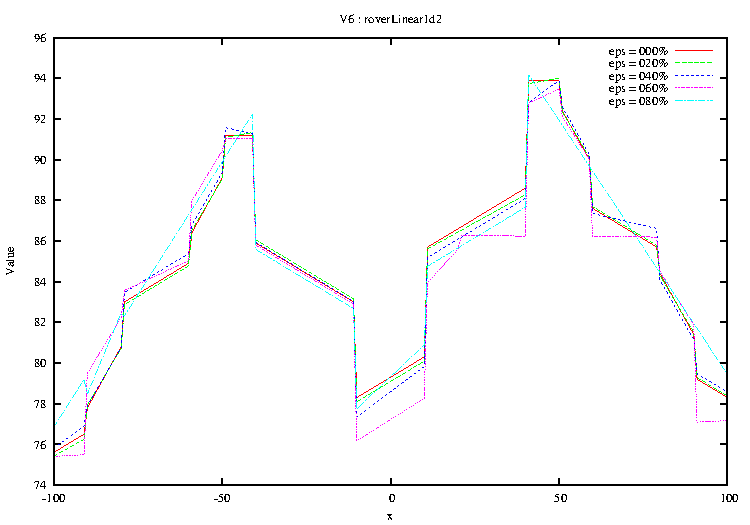
\includegraphics[width=0.45\textwidth]{Figures/rover1D/rover1d2V6.pdf} 
\caption{Value Function at Iteration 6 for rover1d2.}
\label{steplin} 
\end{figure}

\MarsRoverBi: In this version of \MarsRover ~there are no picture points but the rover is expected to follow a path. The position is represented by a pair or continuous variables $(x,y)$. There is only one action, $move(a_x,a_y)$, where $|a_x|$ <10 and $|a_x|$ <10. The new position is given by $(x',y') = ( x+a_x, y+a_y)$. The reward increases with $x$ and decreases with the absolute value of $y$, that is:
{\footnotesize
\begin{align*}
R & = \begin{cases}
(x > y +25) \wedge (x > - y  +25) \wedge (y >0): &-10 + x -y\\
(x > y +25) \wedge (x > - y  +25) \wedge (y <0): & -10 + x +y\\
else: & -1\\
\end{cases}
\end{align*}}

\begin{figure*}[tbph!]
\centering
\subfigure[Value at $6^{th}$ iteration for exact SDP.] {
	 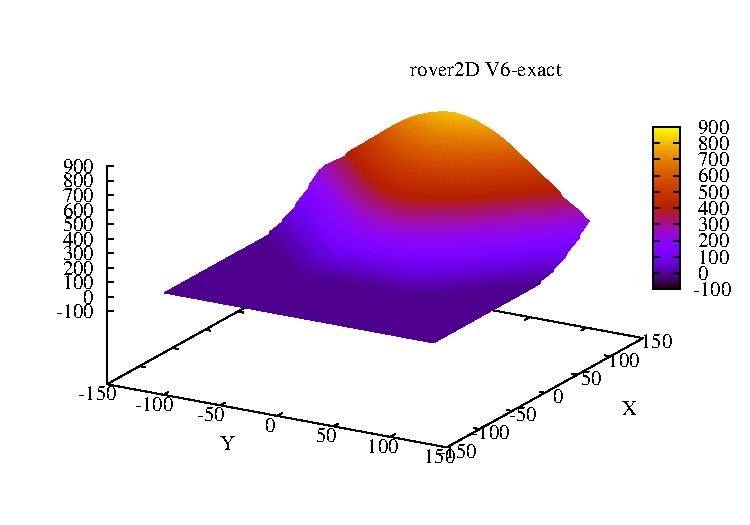
\includegraphics[width=0.45\textwidth, height=0.3\textwidth]{Figures/rover2D/rover2dV6-0.pdf}
	 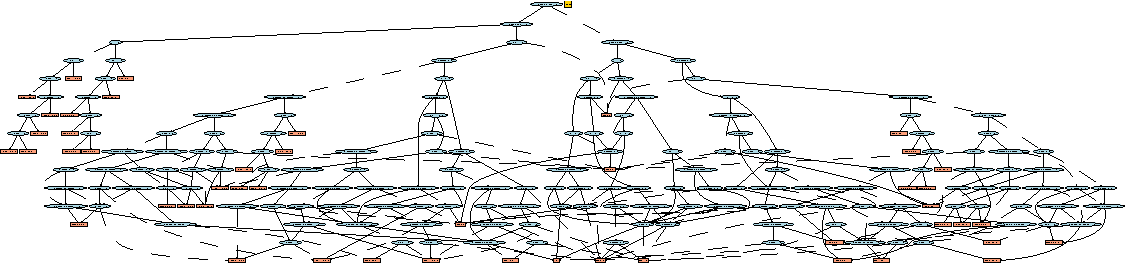
\includegraphics[width=0.45\textwidth, height=0.3\textwidth]{Figures/rover2D/rover2dV6-0xadd.pdf}
	 \label{V6-0xadd}
}
\subfigure[Value at $6^{th}$ iteration for $5\%$ approximate SDP.] {
	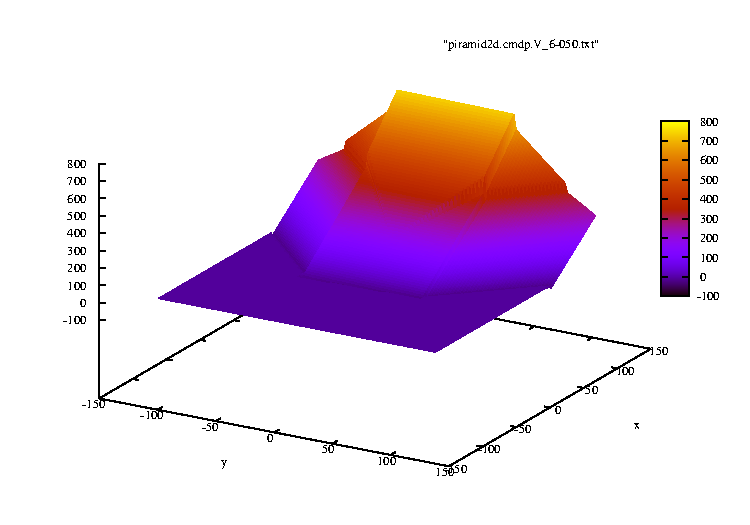
\includegraphics[width=0.45\textwidth, height=0.3\textwidth]{Figures/rover2D/rover2dV6-5.pdf}
	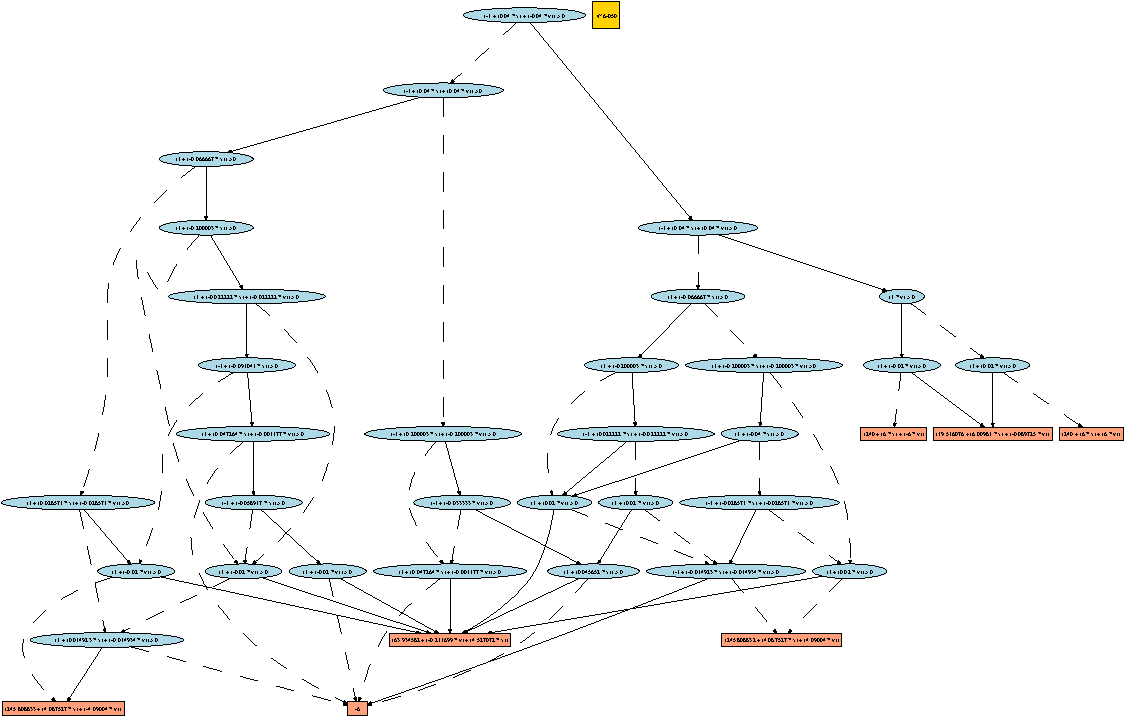
\includegraphics[width=0.45\textwidth, height=0.3\textwidth]{Figures/rover2D/rover2dV6-5xadd.pdf}
	 \label{V6-5xadd}
}
\caption {\footnotesize
	Value function at iteration 6 for the \MarsRoverBi domain;
	{\it (top)} Exact value function; 	{\it (bottom)} Approximate value function with error bounded 5\% per iteration;
	{\it (right)} 3D Plots; {\it (left) XADD Diagrams}.
}
\label{fig:Mars2DV6}
\vspace{-5mm}
\end{figure*}

\begin{figure*}[tbph!]
\centering
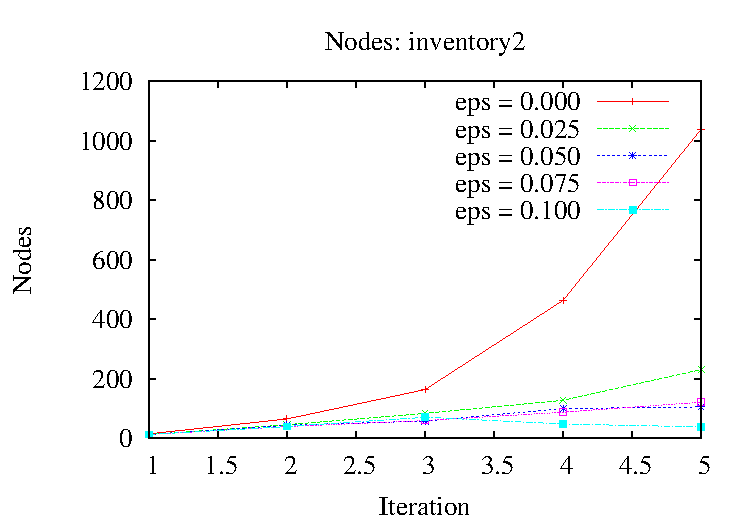
\includegraphics[width=0.32\textwidth]{Figures/inventory/inventory2Nodes.pdf}
\hspace{1mm}
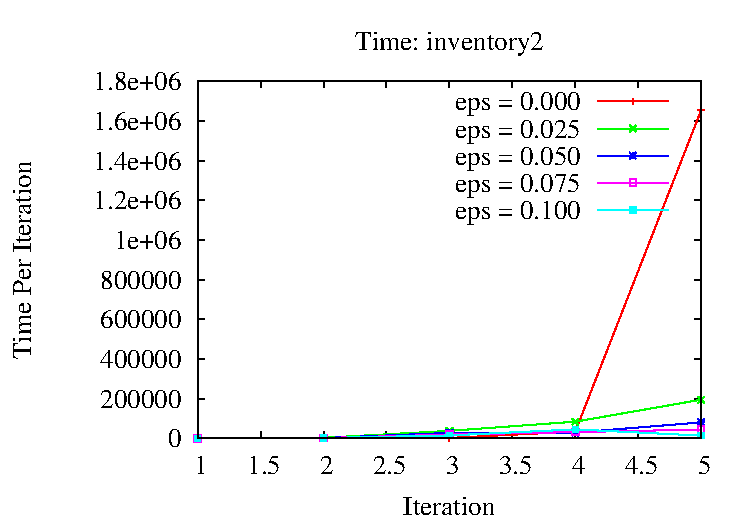
\includegraphics[width=0.32\textwidth]{Figures/inventory/inventory2Time.pdf}
\hspace{1mm}
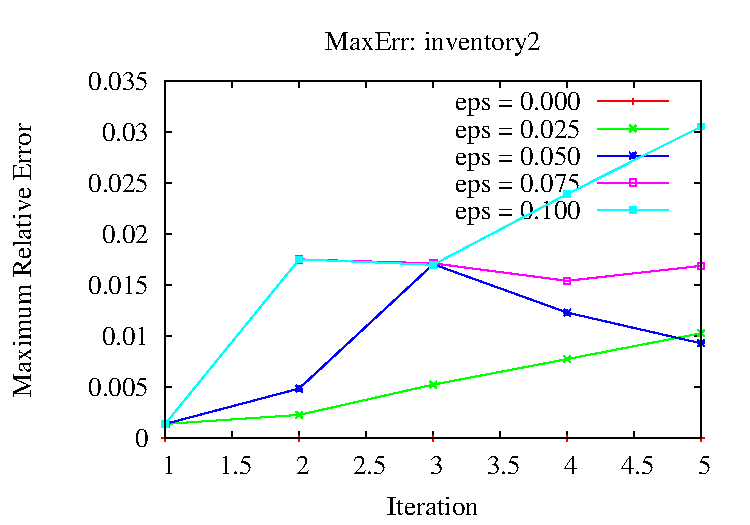
\includegraphics[width=0.32\textwidth]{Figures/inventory/inventory2MaxErr.pdf}
\\
\vspace{5mm}
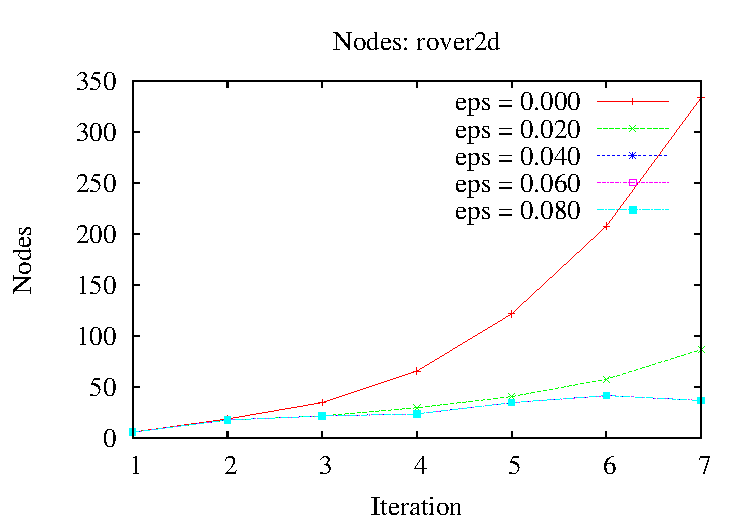
\includegraphics[width=0.32\textwidth]{Figures/rover2D/rover2d-Nodes.pdf}
\hspace{1mm}
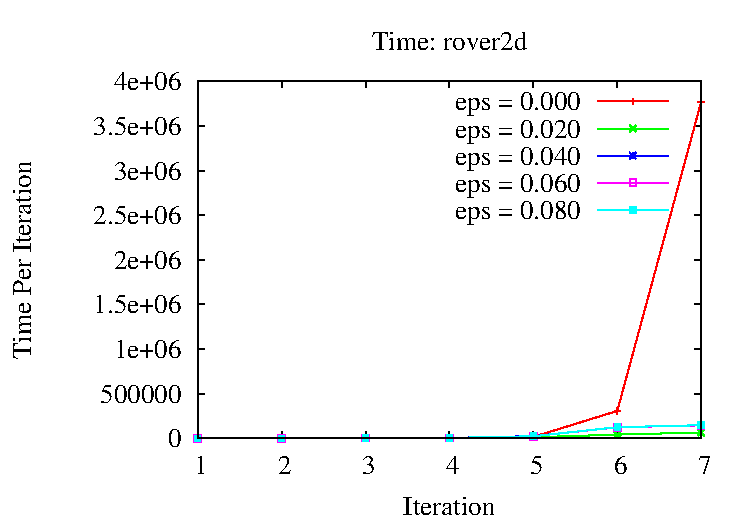
\includegraphics[width=0.32\textwidth]{Figures/rover2D/rover2d-Time.pdf}
\hspace{1mm}
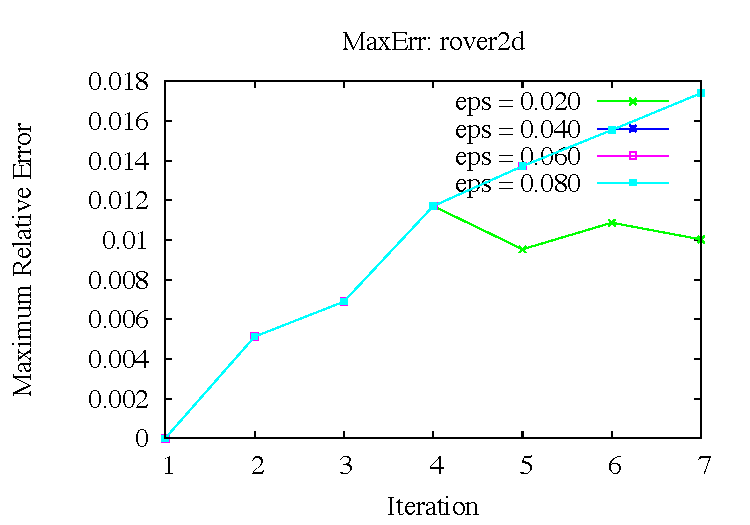
\includegraphics[width=0.32\textwidth]{Figures/rover2D/rover2d-MaxErr.pdf}
\caption{\footnotesize Performance plots for $\MarsRover$ and $\Invent$2 with 5 different relative errors (eps):
{\it (left)}  Space (number of Nodes);
{\it (middle)} Time (miliseconds);
{\it (right)} Maximal error as fraction of the max value.
}
\label{fig:Value}
\vspace{-5mm}
\end{figure*}


\Invent:
A multidimensional continuous, in $n$-$\Invent$. There are $n$ continuous resources that can be bought and sold. There are $n$ non-parametric actions $order$-$i$ for each resource, $ 1 \leq i \leq n$. The maximum amount of  each resource that is sold on one iteration depends on a stochastic demand variable $d$ that is true with $60\%$ probability. The resource $x_i'$ for action $order$-$i$ is given by:
{\footnotesize
\begin{align*}
x_i' & = \begin{cases} 
(d') \wedge (x_i > 150) &: x_i + 200 - 150\\
(d') \wedge (x_i < 150) &:  200\\
(\neg d') \wedge (x_i > 50) &: x_i + 200 - 50\\
(\neg d') \wedge (x_i < 50) &:  200\\
\end{cases} \\
\end{align*} }
and for other resources $x_j'$, $1 \leq j \leq n$, $j\neq i$:\\
{\footnotesize
\begin{align*}
x_j' & = \begin{cases} 
(d') \wedge (x_j > 150) &: x_j - 150\\
(d') \wedge (x_j < 150) &:  0\\
(\neg d') \wedge (x_j > 50) &: x_j - 50\\
(\neg d') \wedge (x_j < 50) &:  0\\
\end{cases} \\
R & = \begin{cases} \\
(d') &: \sum_{k} {x_k' - x_k}\\
(tp1') \wedge (\neg tp1) \wedge (x < 50) &: 40 - 0.2*(50-x)\\
(tp1') \wedge ( tp1) &:  1.1\\
else & -2\\
\end{cases} 
\end{align*} }


Figure \ref{fig:Value} shows the results of exact and approximate solutions for two domains. In the left plots we notice how the approximation does compress the XADD significantly. The remaining plots, show that the compression results in faster computation while never exceeding the allowed error.
